\begin{figure}[H]
  \centering
  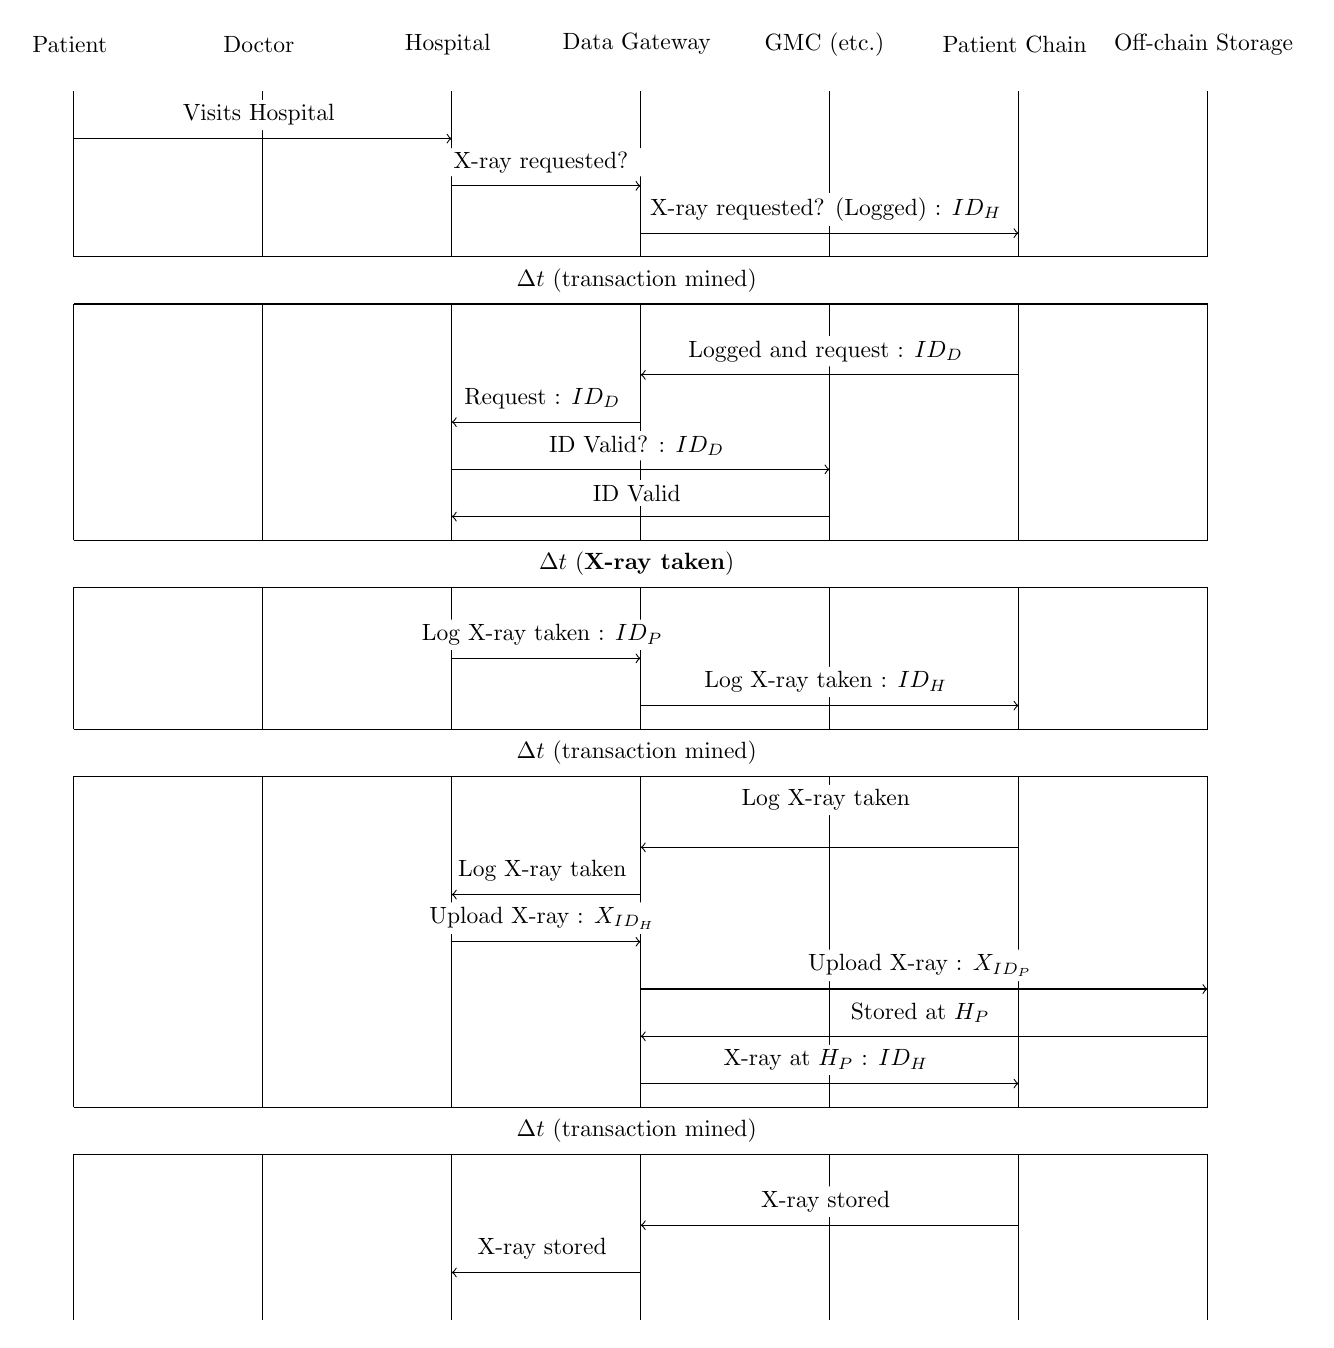
\begin{tikzpicture}[scale = 0.6, every node/.style={scale = 0.85}, every node/.append style={fill = white, rounded corners = 2pt, inner sep = 2pt, align = center}]

  % Lines
  \draw (4, -6) -- (4, -2.5);
  \draw (4, -1.5) -- (4, 5.5);
  \draw (4, 6.5) -- (4, 9.5);
  \draw (4, 10.5) -- (4, 15.5);
  \draw (4, 16.5) -- (4, 20);
  \draw (8, -6) -- (8, -2.5);
  \draw (8, -1.5) -- (8, 5.5);
  \draw (8, 6.5) -- (8, 9.5);
  \draw (8, 10.5) -- (8, 15.5);
  \draw (8, 16.5) -- (8, 20);
  \draw (12, -6) -- (12, -2.5);
  \draw (12, -1.5) -- (12, 5.5);
  \draw (12, 6.5) -- (12, 9.5);
  \draw (12, 10.5) -- (12, 15.5);
  \draw (12, 16.5) -- (12, 20);
  \draw (16, -6) -- (16, -2.5);
  \draw (16, -1.5) -- (16, 5.5);
  \draw (16, 6.5) -- (16, 9.5);
  \draw (16, 10.5) -- (16, 15.5);
  \draw (16, 16.5) -- (16, 20);
  \draw (20, -6) -- (20, -2.5);
  \draw (20, -1.5) -- (20, 5.5);
  \draw (20, 6.5) -- (20, 9.5);
  \draw (20, 10.5) -- (20, 15.5);
  \draw (20, 16.5) -- (20, 20);
  \draw (24, -6) -- (24, -2.5);
  \draw (24, -1.5) -- (24, 5.5);
  \draw (24, 6.5) -- (24, 9.5);
  \draw (24, 10.5) -- (24, 15.5);
  \draw (24, 16.5) -- (24, 20);
  \draw (28, -6) -- (28, -2.5);
  \draw (28, -1.5) -- (28, 5.5);
  \draw (28, 6.5) -- (28, 9.5);
  \draw (28, 10.5) -- (28, 15.5);
  \draw (28, 16.5) -- (28, 20);

  % Headings
  \node at (4, 21) { Patient };
  \node at (8, 21) { Doctor };
  \node at (12, 21) { Hospital };
  \node at (16, 21) { Data Gateway };
  \node at (20, 21) { GMC (etc.) };
  \node at (24, 21) { Patient Chain };
  \node at (28, 21) { Off-chain Storage };

  % Arrows
  \node at (8, 19.5) { Visits Hospital };
  \draw [ -> ] (4, 19) -- (12, 19);

  \node at (14, 18.5) { X-ray requested? };
  \draw [ -> ] (12, 18) -- (16, 18);

  \node at (20, 17.5) { X-ray requested? (Logged) : $ID_{H}$ };
  \draw [ -> ] (16, 17) -- (24, 17);

  \draw (4, 16.5) -- (28, 16.5);
  \node at (16, 16) { $\Delta t$ (transaction mined) };
  \draw (4, 15.5) -- (28, 15.5);

  \node at (20, 14.5) { Logged \checkmark and request : $ID_{D}$ };
  \draw [ -> ] (24, 14) -- (16, 14);

  \node at (14, 13.5) { Request : $ID_{D}$ };
  \draw [ -> ] (16, 13) -- (12, 13);

  \node at (16, 12.5) { ID Valid? : $ID_{D}$ };
  \draw [ -> ] (12, 12) -- (20, 12);

  \node at (16, 11.5) { ID Valid \checkmark };
  \draw [ -> ] (20, 11) -- (12, 11);

  \draw (4, 10.5) -- (28, 10.5);
  \node at (16, 10) { $\Delta t$ (\textbf{X-ray taken}) };
  \draw (4, 9.5) -- (28, 9.5);

  \node at (14, 8.5) { Log X-ray taken : $ID_{P}$ };
  \draw [ -> ] (12, 8) -- (16, 8);

  \node at (20, 7.5) { Log X-ray taken : $ID_{H}$ };
  \draw [ -> ] (16, 7) -- (24, 7);

  \draw (4, 6.5) -- (28, 6.5);
  \node at (16, 6) { $\Delta t$ (transaction mined) };
  \draw (4, 5.5) -- (28, 5.5);

  \node at (20, 5) { Log X-ray taken \checkmark };
  \draw [ -> ] (24, 4) -- (16, 4);

  \node at (14, 3.5) { Log X-ray taken \checkmark };
  \draw [ -> ] (16, 3) -- (12, 3);

  \node at (14, 2.5) { Upload X-ray : $X_{ID_{H}}$ };
  \draw [ -> ] (12, 2) -- (16, 2);

  \node at (22, 1.5) { Upload X-ray : $X_{ID_{P}}$ };
  \draw [ -> ] (16, 1) -- (28, 1);

  \node at (22, 0.5) { Stored at $H_{P}$ };
  \draw [ -> ] (28, 0) -- (16, 0);

  \node at (20, -0.5) { X-ray at $H_{P}$ : $ID_{H}$ };
  \draw [ -> ] (16, -1) -- (24, -1);

  \draw (4, -1.5) -- (28, -1.5);
  \node at (16, -2) { $\Delta t$ (transaction mined) };
  \draw (4, -2.5) -- (28, -2.5);

  \node at (20, -3.5) { X-ray stored \checkmark };
  \draw [ -> ] (24, -4) -- (16, -4);

  \node at (14, -4.5) { X-ray stored \checkmark };
  \draw [ -> ] (16, -5) -- (12, -5);

  \end{tikzpicture}
  \caption{
    Patient visits hospital to have X-ray taken
  }
  \label{fig:user_story_02}
\end{figure}
